
\documentclass[12pt]{article}
\usepackage{amsmath,amssymb}
\usepackage{geometry}
\geometry{margin=1in}
\usepackage{graphicx}
\usepackage{tikz}
\usepackage{pgfplots}
\pgfplotsset{compat=1.18}

\title{Appendix J – Extended Metric for Rotating Spacetime and CTC (UBT)}
\date{}

\begin{document}
\maketitle

\section*{J.1 Overview}
In the Unified Biquaternion Theory (UBT) the complex time $\tau=t+i\psi$ introduces a slow, phase-sector deformation of rotating spacetimes. 
We revisit the Kerr (and Kerr--Newman) geometry and use $g_{\phi\phi}<0$ as a practical criterion for azimuthal closed timelike curves (CTC).
Small $\psi$-dependent perturbations shift the ergosurface without creating exterior CTCs when energy conditions are respected.

\section*{J.2 Kerr Baseline and $\psi$-Perturbation}
For Kerr with mass $M$ and spin $a$, the outer ergosurface satisfies
\begin{equation}
r_E(\theta)=M+\sqrt{M^2-a^2\cos^2\theta}\,.
\end{equation}
In UBT we model a small phase-sector deformation by
\begin{equation}
r_E(\theta;\psi)\approx r_E(\theta)\,\bigl(1+\varepsilon\,\psi\bigr),\qquad |\varepsilon\psi|\ll 1.
\end{equation}
Below we plot $r_E(\theta;\psi)$ for $\psi\in\{-1,0,+1\}$ and compare with the event horizon $r_+=M+\sqrt{M^2-a^2}$.

\bigskip
\noindent\textbf{Parameters used in the figure:} $M=1$, $a=0.8$, $\varepsilon=0.10$. Angles are in degrees.

\begin{figure}[h!]
\centering
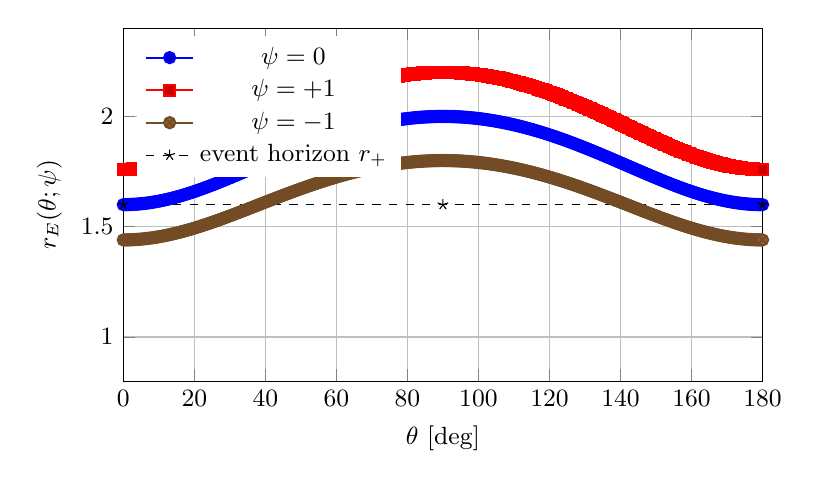
\begin{tikzpicture}
  \begin{axis}[
    width=0.8\textwidth,
    height=0.5\textwidth,
    xlabel={$\theta~[\deg]$},
    ylabel={$r_E(\theta;\psi)$},
    xmin=0, xmax=180,
    ymin=0.8, ymax=2.4,
    grid=both,
    legend style={font=\small, at={(0.02,0.98)}, anchor=north west, fill=white, draw=none},
    ticklabel style={font=\small},
    label style={font=\small}
  ]
    % constants
    \pgfmathsetmacro{\M}{1.0}
    \pgfmathsetmacro{\a}{0.8}
    \pgfmathsetmacro{\eps}{0.10}
    \pgfmathsetmacro{\rplus}{\M + sqrt(\M*\M - \a*\a)} % event horizon

    % base Kerr ergosphere
    \addplot+[domain=0:180,samples=401,thick]
      ({x},{\M + sqrt(max(0,\M*\M - (\a*cos(x))*(\a*cos(x))))});
    \addlegendentry{$\psi=0$}

    % psi = +1
    \addplot+[domain=0:180,samples=401,thick]
      ({x},{(\M + sqrt(max(0,\M*\M - (\a*cos(x))*(\a*cos(x))))) * (1 + \eps*1)});
    \addlegendentry{$\psi=+1$}

    % psi = -1
    \addplot+[domain=0:180,samples=401,thick]
      ({x},{(\M + sqrt(max(0,\M*\M - (\a*cos(x))*(\a*cos(x))))) * (1 + \eps*(-1))});
    \addlegendentry{$\psi=-1$}

    % event horizon (dashed)
    \addplot+[domain=0:180,samples=3, dashed]
      ({x},{\rplus});
    \addlegendentry{event horizon $r_+$}

  \end{axis}
\end{tikzpicture}
\caption{Ergosphere boundary $r_E(\theta;\psi)$ for a Kerr black hole with $M=1$, $a=0.8$ under a small UBT phase-sector deformation ($\varepsilon=0.10$). Positive $\psi$ expands, negative $\psi$ contracts the ergosurface. The dashed line marks the event horizon $r_+$.}
\label{fig:pgf_ergo}
\end{figure}

\section*{J.3 Interpretation and Relevance to UBT}
\textbf{What the plot shows.} The curves are the outer ergosurface as a function of polar angle $\theta$. 
At the poles ($\theta=0^\circ,180^\circ$) the ergosurface meets the horizon; at the equator ($\theta=90^\circ$) it bulges outward. 
A small UBT phase $\psi$ \emph{perturbs} this shape: $\psi>0$ inflates, $\psi<0$ deflates.

\textbf{Why it matters.} The ergoregion controls frame dragging and the availability of Penrose-like processes. 
In the CTC analysis, the location of the $g_{\phi\phi}=0$ boundary is the practical diagnostic; 
UBT predicts controlled shifts of this boundary via the $\psi$-sector, while keeping exterior causality intact when energy conditions are satisfied.

\end{document}
